\newpage
	\section*{Aufgabe 3}
	\graphicspath{{D:/GoogleDrive/UNI/SZS/Blatt1/3/}{D:/GoogleDrive/UNI/SZS/Blatt1/4/}}

\subsection*{b)}

\begin{minipage}[h]{0.5\textwidth}
	\centering
	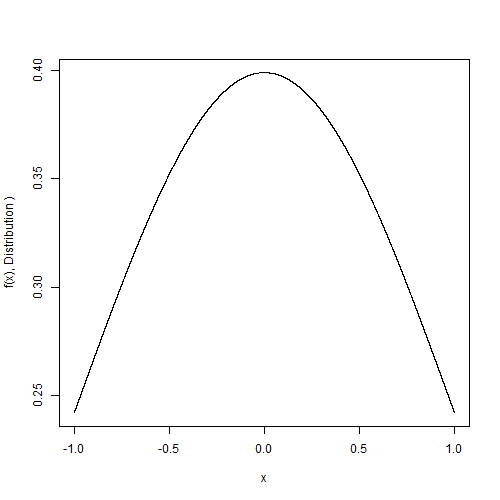
\includegraphics[width=0.8\textwidth]{bDistribution.png} 	
\end{minipage}\begin{minipage}[h]{0.5\textwidth}
	\centering
	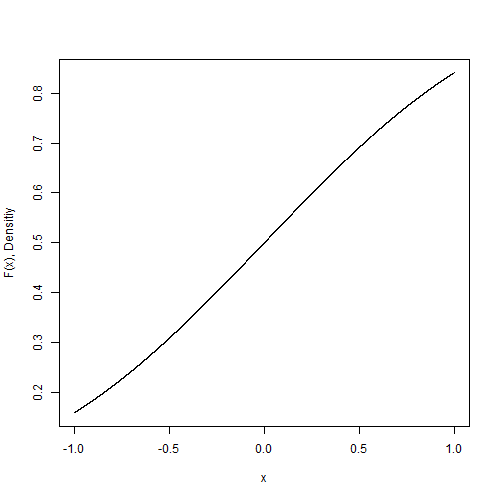
\includegraphics[width=0.8\textwidth]{bDensity.png}
\end{minipage}

\subsection*{c)}

\begin{minipage}[h]{0.5\textwidth}
	\centering
	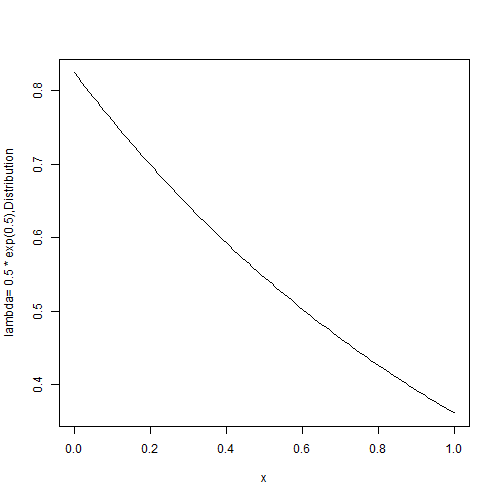
\includegraphics[width=0.8\textwidth]{c1.png} 
	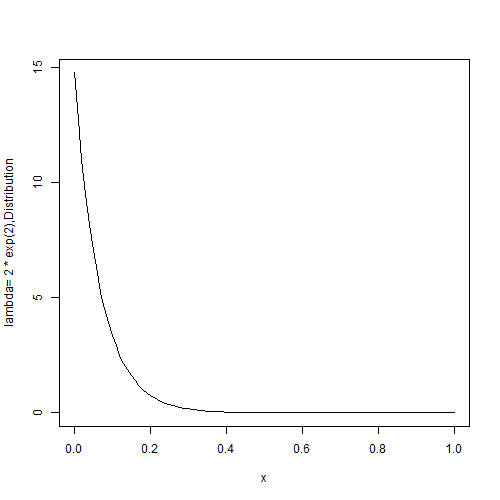
\includegraphics[width=0.8\textwidth]{c3.png} 		
\end{minipage}\begin{minipage}[h]{0.5\textwidth}
	\centering
	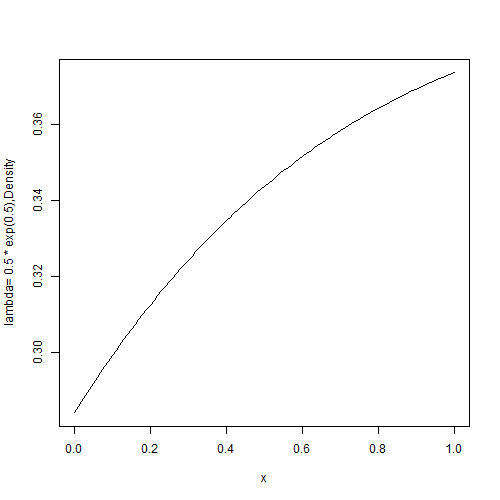
\includegraphics[width=0.8\textwidth]{c2.png}
	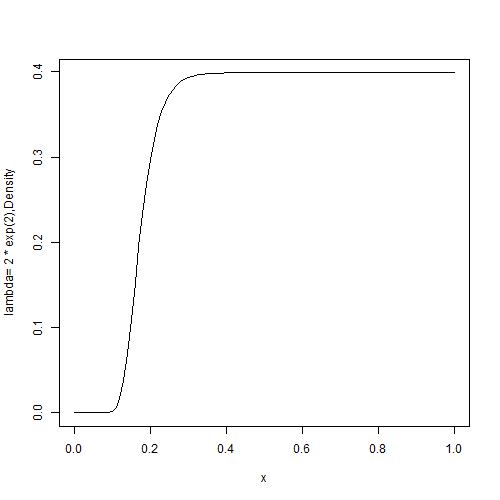
\includegraphics[width=0.8\textwidth]{c4.png} 	
\end{minipage}

\subsection*{d)}
\begin{minipage}[h]{0.5\textwidth}
	\centering
	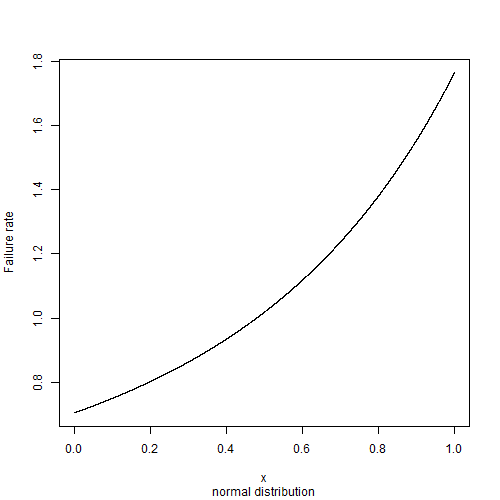
\includegraphics[width=0.8\textwidth]{dnorm.png}
	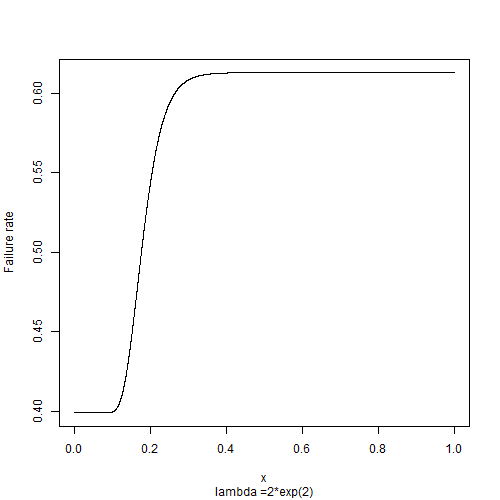
\includegraphics[width=0.8\textwidth]{d2.png}		
\end{minipage}\begin{minipage}[h]{0.5\textwidth}
	\centering
	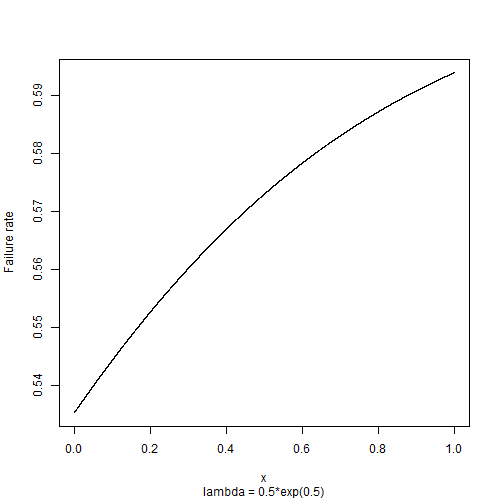
\includegraphics[width=0.8\textwidth]{d05.png} 	
\end{minipage}

\subsection*{e)}
Am letzten Diagramm kann man die Unabhängigkeit von x sehr gut erkennen.
die Failure rate ist im bereich 0.4-1 konstant obwohl sich x ändert.

\section*{Aufgabe 4}

	\subsection*{a)}
	 \begin{center}
	 	Max = 1633 , Min = 0 , Avg = 1026,867
	 \end{center}
	\subsection*{b)}
		\centering
		$P(1200 \leq X \leq 1400) = \frac{\#DaysWithinRange}{\#TotalDays}=\frac{5}{30} = 0.1\overline{6} = 16,\overline{6}\%$ 
		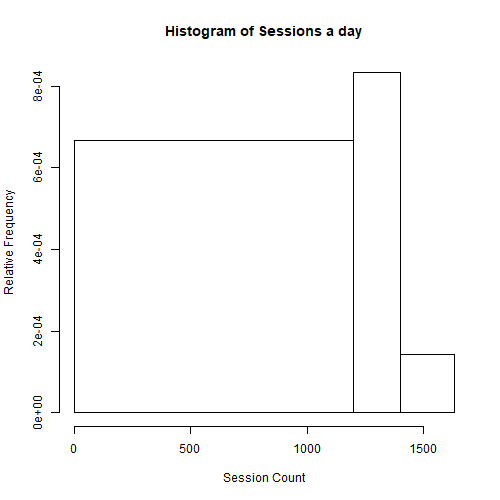
\includegraphics[width=0.5\textwidth]{4histo.png}\\
		Breaks used: 0,1200,1400,163
	\newpage
	\subsection*{c)}
		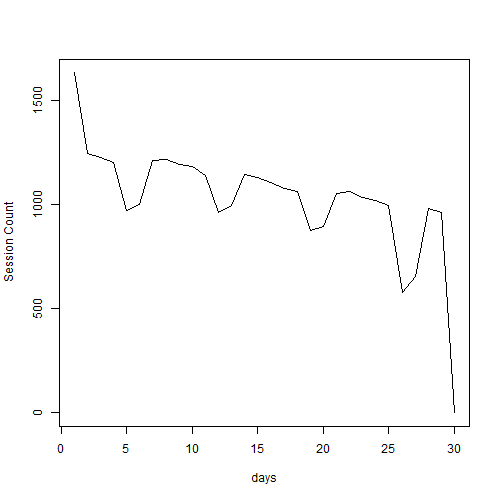
\includegraphics[width=0.5\textwidth]{distr.png}\\
		Am Tag 1 ist die Spitzenlast bereits erreicht.
		Durch das benutzen von zeitlich enger zusammen liegenden Messpunkten würde sich der Zeitpunkt in dem die Spitzenlast genauer bestimmen lassen. Je nachdem wie man die Spitzenlast vorher bestimmt hat könnt sie sinken (durch Verteilung auf kleinere Abschnitte) oder steigen (Registrierung von Sessions, die zwischen den vorherigen Messpunkten lagen.).
		
		
	
	
	
	
	
	
	
	